\documentclass[a4paper,12pt,obeyspaces,spaces,hyphens]{article}

\usepackage{agenda}
\usepackage{colortbl}
\usepackage{xcolor}
\usepackage{palatino}
\usepackage{calc}

\hypersetup{pdftitle={Yocto Project and OpenEmbedded development training},
  pdfauthor={Free Electrons}}

\begin{document}

\thispagestyle{fancy}

\setlength{\arrayrulewidth}{0.8pt}

\begin{center}
\LARGE
Yocto Project and OpenEmbedded training\\
\large
3-day session
\end{center}
\vspace{1cm}

\small
\newcolumntype{g}{>{\columncolor{fedarkblue}}m{4cm}}
\newcolumntype{h}{>{\columncolor{felightblue}}X}

\arrayrulecolor{lightgray} {
  \setlist[1]{itemsep=-5pt}
  \begin{tabularx}{\textwidth}{|g|h|}
    {\bf Title} & Yocto Project and OpenEmbedded development training \\
    \hline

    {\bf Overview} &
    Understanding the Yocto Project \par
    Using it to build a root filesystem and run it on your target \par
    Writing and extending recipes \par
    Creating layers \par
    Integrating your board in a BSP \par
    Creating custom images \par
    Application development with an Eclipse SDK \\
    \hline

    {\bf Duration} & {\bf Three} days - 24 hours (8 hours per day).
    \newline 40\% of lectures, 60\% of practical labs. \\
    \hline

    {\bf Trainer} & One of the engineers listed on
    \newline \url{http://free-electrons.com/training/trainers/}\\
    \hline

    {\bf Language} & Oral lectures: English, French.
    \newline Materials: English.\\
    \hline

    {\bf Audience} & Companies interested in using the Yocto Project to build their
    embedded Linux system.\\
    \hline

    {\bf Prerequisites} & {\bf Knowledge of embedded Linux} as covered
    in our embedded Linux training
    (\url{http://free-electrons.com/training/embedded-linux/}) \newline 
    {\bf Knowledge and practice of Unix or GNU/Linux commands}
    \newline People lacking experience on this topic should get
    trained by themselves with our freely available on-line slides
    (\url{http://free-electrons.com/docs/command-line/}) \\
    \hline

    {\bf Required equipment} &
    {\bf For on-site sessions only.}
    \newline Everything is supplied by Free Electrons in public
    sessions.
    \begin{itemize}
    \item Video projector
    \item PC computers with at least 4 GB of RAM, a CPU at least
      equivalent to an Intel Core i5 and Ubuntu Linux
    installed in a {\bf free partition of at least 20 GB. Using Linux
      in a virtual machine is not supported}, because of issues
    connecting to real hardware.
    \item We need Ubuntu Desktop 12.04 (32 or 64 bit, Xubuntu and
    Kubuntu variants are fine). We don't support other
    distributions, because we can't test all possible package versions.
    \item {\bf High Speed Connection to the Internet} (direct or through the
    company proxy).
    \item {\bf PC computers with valuable data must be backed up}
    before being used in our sessions.  Some people have already made
    mistakes during our sessions and damaged work data.
    \end{itemize} \\
    \hline

    {\bf Materials} & Print and electronic copies of presentations and
    labs.
    \newline Electronic copy of lab files.\\
    \hline

\end{tabularx}}
\normalsize

\feagendatwocolumn
{Hardware}
{
  The hardware platform used for the practical labs of this training
  session is the {\bf BeagleBone Black board}, which features:

  \begin{itemize}
  \item An ARM AM335x processor from Texas Instruments (Cortex-A8
    based), 3D acceleration, etc.
  \item 512 MB of RAM
  \item 2 GB of on-board eMMC storage
  \item USB host and device
  \item HDMI output
  \item 2 x 46 pins headers, to access UARTs, SPI busses, I2C busses
    and more.
  \end{itemize}
}
{}
{
  \begin{center}
    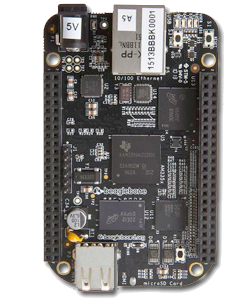
\includegraphics[height=5cm]{agenda/beagleboneblack.png}
  \end{center}
}

\section{Day 1 - Morning}

\feagendaonecolumn
{Lecture - Introduction to embedded Linux build systems}
{
  \begin{itemize}
  \item Overview of an embedded Linux system architecture
  \item Methods to build an image
  \item Usefulness of build systems
  \end{itemize}
}
\\
\feagendatwocolumn
{Lecture - Overview of the Yocto Project and the Poky reference system}
{
  \begin{itemize}
  \item Organization of the project source tree
  \item Building an image using the project
  \end{itemize}
}
{Lab - First Yocto Project build}
{
  \begin{itemize}
  \item Downloading the Poky reference build system
  \item Building a system image
 \end{itemize}
}

\section{Day 1 - Afternoon}
\feagendatwocolumn
{Lecture - Using Yocto Project - basics}
{
  \begin{itemize}
  \item Organization of the build output
  \item Flashing and installing the image
  \end{itemize}
}
{Lab - Flashing and booting}
{
  \begin{itemize}
  \item Flashing and booting the image on the BeagleBone
  \end{itemize}
}

\feagendatwocolumn
{Lecture - Using Yocto Project - advanced usage}
{
  \begin{itemize}
  \item Configuring the build system
  \item Customizing the package selection
  \end{itemize}
}
{Lab - Using NFS and configuring the build}
{
  \begin{itemize}
  \item Configuring the BeagleBone to boot over NFS
  \item Learn how to use the \code{PREFERRED_PROVIDER} mechanism
  \end{itemize}
}
\\
\section{Day 2 - Morning}

\feagendatwocolumn
{Lecture - Writing recipes - basics}
{
  \begin{itemize}
  \item Writing a minimal recipe
  \item Adding dependencies
  \item Development workflow with bitbake
  \end{itemize}
}
{Lab - Adding an application to the build}
{
  \begin{itemize}
  \item Writing a recipe for nInvaders
  \item Adding nInvaders to the final image
  \end{itemize}
}

\feagendaonecolumn
{Lecture - Writing recipes - advanced features}
{
  \begin{itemize}
  \item Extending and overriding recipes
  \item Adding steps to the build process
  \item Learn about classes
  \item Analysis of examples
  \item Logging
  \item Debugging dependencies
  \end{itemize}
}

\section{Day 2 - Afternoon}

\feagendaonecolumn
{Lab - Learning how to configure packages}
{
  \begin{itemize}
  \item Extending a recipe to add configuration files
  \item Using \code{ROOTFS_POSTPROCESS_COMMAND} to modify the final rootfs
  \item Studying package dependencies
  \end{itemize}
}
\feagendatwocolumn
{Lecture - Layers}
{
  \begin{itemize}
  \item What layers are
  \item Where to find layers
  \item Creating a layer
  \end{itemize}
}
{Lab - Writing a layer}
{
  \begin{itemize}
  \item Learn how to write a layer
  \item Add the layer to the build
  \item Move nIvaders to the new layer
  \end{itemize}
}

\section{Day 3 - Morning}

\feagendatwocolumn
{Lecture - Writing a BSP}
{
  \begin{itemize}
  \item Extending an existing BSP
  \item Adding a new machine
  \item Bootloaders
  \item Linux and the linux-yocto recipe
  \item Adding a custom image type
  \end{itemize}
}
{Lab - Implementing the kernel changes}
{
  \begin{itemize}
  \item Extend the kernel recipe to add the nunchuk driver
  \item Configure the kernel to include the nunchuk driver
  \item Play nInvaders
  \end{itemize}
}

\section{Day 3 - Afternoon}

\feagendatwocolumn
{Lecture - Creating a custom image}
{
  \begin{itemize}
  \item Writing an image recipe
  \item Adding users/groups
  \item Adding custom configuration
  \item Writing and using package groups recipes
  \end{itemize}
}
{Lab - Creating a custom image}
{
  \begin{itemize}
  \item Writing a custom image recipe
  \item Adding nInvader to the custom image
  \end{itemize}
}
\feagendatwocolumn
{Lecture - Creating and using an SDK}
{
  \begin{itemize}
  \item Understanding the purpose of an SDK for the application
    developer
  \item Building an SDK for the custom image
  \end{itemize}
}
{Lab - Experimenting with the SDK}
{
  \begin{itemize}
  \item Building an SDK
  \item Using the SDK through Eclipse
  \end{itemize}
}

\end{document}

